\chapter{The Fundamentals of Cloud Computing}
\label{ch:cloud_computing}

\textit{In the previous chapter the three predominant architectural patterns in design of distributed systems were described. It was concluded that the microservice architecture serves as a great architecture for creating resilient systems. The ideas behind microservice are grounded in cloud computing it is in this space many of the technologies enabling microservices have been developed. This chapter will therefore explain the possibilities cloud computing has created for development and distribution of applications, as well as the cloud native movement behind it, pushing companies towards microservice architectures.}

Cloud computing is both applications available on the internet, but also the hardware and system software that provide these services.
Rather than scaling a single node vertically, Cloud computing shifts focus and enables horizontal scaling of virtualized storage and network resources \cite{armbrust2010view}. Cloud computing enable applications to fulfil new requirements for rapid capacity up and down scaling, with the notion that available virtual resources are limitless \cite{sosinsky2010cloud}. At the same time virtualization facilitates reproducibility, resource isolation and transparency, recently revolutionised by the container abstraction, making it possible to create systems consisting of many small independent services. 

According to Sosinsky \cite[p. 3 ]{sosinsky2010cloud}, cloud computing sets new standards for system development and deployment, representing a real paradigm shift:

\tquote{Cloud computing represents a real paradigm shift in the way in which systems are deployed. The massive scale of cloud computing systems was enabled by the popularization of the Internet and the growth of some large service companies. Cloud computing makes the long-held dream of utility computing possible with a pay-as-you-go, infinitely scalable, universally available system. [...] That’s why cloud computing is revolutionary, even if the technology it is built on is evolutionary}{Sosinsky}{2010}

Cloud computing is an enabler for further evolving how distributed systems are designed, distributed, updated and accessed. 

\section{Defining Cloud Computing}
This section will try to pin down what defines cloud computing, determining a concise meaning for the term.

The National Institute of Standards and Technology (NIST) has defined cloud computing \cite{mell2011nist}:

\defi{Cloud Computing (NIST)}{Cloud computing is a model for enabling ubiquitous, convenient, on-demand network access to a shared pool of configurable computing resources}{The NIST definition of cloud computing\cite{mell2011nist}}

NIST characterizes cloud computing as an infrastructure that through a composition of hardware and software enable five essential characteristics:

\textbf{On-demand self-service}\\
Computing capabilities can be provisioned on-demand automatically without human interaction.

\textbf{Broad network access}\\
Capabilities are heterogeneous accessible over the network.

\textbf{Resource pooling}\\
The providers computing resources are pooled, serving multiple consumers simultaneously. Different physical and virtual resources are dynamically assigning and reassigning based on consumer demand.

\textbf{Rapid elasticity}\\
Capabilities are elastic, supporting rapid outward and inward scaling. 

\textbf{Measured service}\\
Resources are measured, providing transparency for both the provider and consumer. Enabling cloud systems to optimize resource usage.

\subsection{Service Models}
The cloud infrastructure is made available to the consumer through three different service models \cite{mell2011nist}. Service models are distinguished by the provided systems software abstraction and resource management level. The level of abstraction and resource management affect the available services, leaving increasing levels of management responsibilities to the provider \cite[p. 52]{armbrust2010view}.
The three service models are depicted in Figure \ref{fig:cloud_computing_definition_service_models} where the different abstraction levels are visible.

\textbf{Software as a Service (SaaS)}\\
The provider makes the complete application available on the cloud infrastructure, for consumers to start up. The applications are accessible through thin client interfaces (eg. web browsers) or program interfaces. The consumer does not manage or control the underlying infrastructure and is therefore alleviated the burden of maintenance, operation and support costs \cite{youseff2008toward}.


\textbf{Platform as a Service (PaaS)}\\
The consumer can deploy consumer-created or acquired applications, controlling the deployment and potentially configuration settings for the hosting environment. Underlying cloud infrastructure network, server storage, virtualization, operating system (OS) and runtime are provider managed \cite{youseff2008toward}.

\textbf{Infrastructure as a Service (IaaS)}\\
The consumer can provision processing, storage and network resources, but does not manage them. The consumer can run arbitrary software \cite{youseff2008toward}.

\begin{figure}[!htb]
  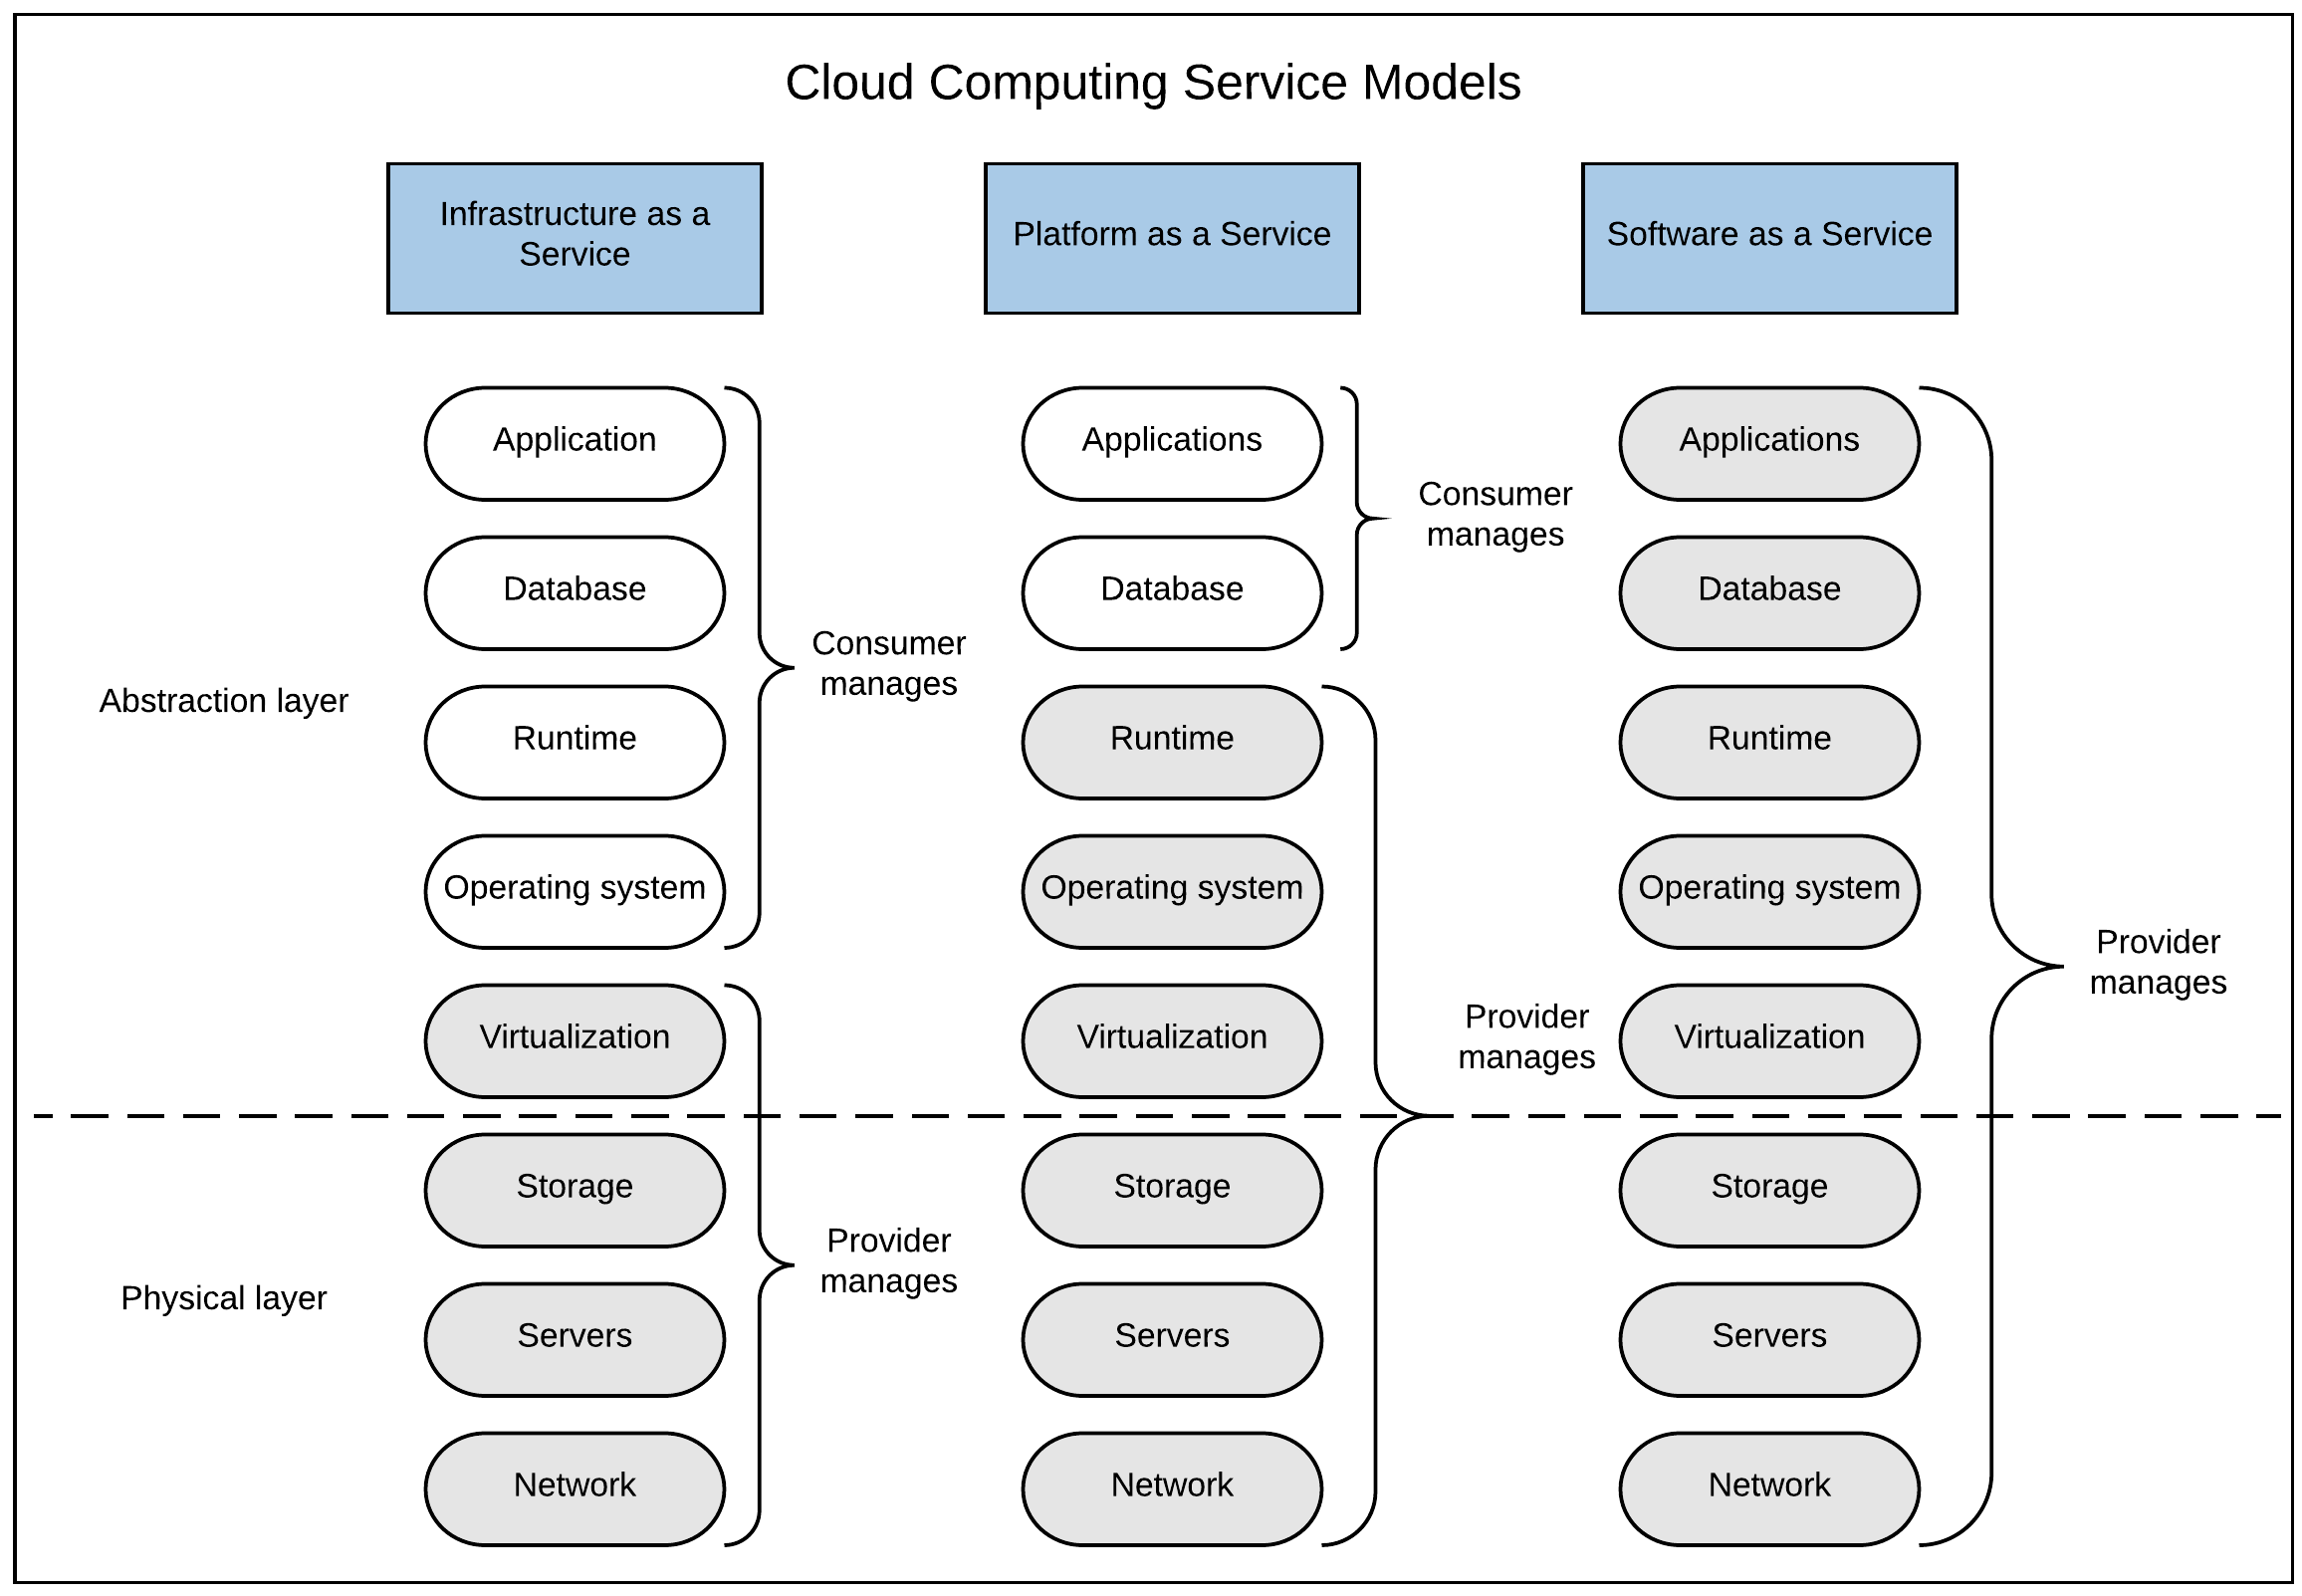
\includegraphics[width=\textwidth]{cloud_computing_definition_service_models}  
  \caption{The three service models providing services at different abstraction levels}
  \label{fig:cloud_computing_definition_service_models}
\end{figure}

This thesis has used the IaaS service model, using the Kubernetes cluster scripts to start the cluster used during experiments, and creating dockerfiles with different types of image types (see section {sec:docker} and \ref{sec:cluster}).

\subsection{Deployment Models}
Cloud infrastructures are made available through four different deployment models with distinct differences. The deployment model describes location and ownership of the infrastructure, determining who is responsible for the infrastructure. The deployment model affects the expected data confidentiality and security, the specified availability and the available deployment size.

\textbf{Private Cloud}\\
Internal data center, provisioned for exclusive use to the owning organization.

\textbf{Community Cloud}\\
The infrastructure is provisioned exclusively to a community of organizations with shared concerns to mission, security and policy etc.

\textbf{Public Cloud}\\
The cloud infrastructure is provisioned to the general public, in a "Pay-as-you-go" manner.

\textbf{Hybrid Cloud}\\
A composition of several distinct cloud infrastructures.


Armbrust et al. states that data confidentiality and auditability is one of the biggest obstacles for a large-scale adoption of public cloud computing infrastructures \cite{armbrust2010view}. Internal consumer concerns and legislation prohibit some consumers from fully adopting public cloud computing infrastructures, forcing a private cloud deployment model, incurring an increased time frame on the adoption of a cloud infrastructure in some enterprises.

\section{Cloud Native Landscape}
The Cloud Native Computing Foundation\footnote{\url{www.cncf.io}} (CNCF) is a foundation that supports the adoption of cloud native computing. They believe that a cloud native application is containerized, dynamically orchestrated and microservice oriented. The purpose of the foundation is to help non-technical companies transition into the cloud. CNCF supports several of the most utilized open source projects in the cloud computing space: Kubernetes and Docker among others.

The Cloud Native Computing Foundation has defined five overall levels in the cloud computing stack: Infrastructure, Provisioning, Runtime, Orchestration \& Management and Application Definition \& Development. This project only involves four of the overall levels in the Cloud Native Landscape definition, seen in Figure \ref{fig:cloud_computing_cloud_native_landscape}. Besides the five overall levels the landscape also contains a Oberservability \& Analysis package. The technologies utilized in this project are shown on each level respectively.

\begin{figure}[!htb]
\begin{center}
  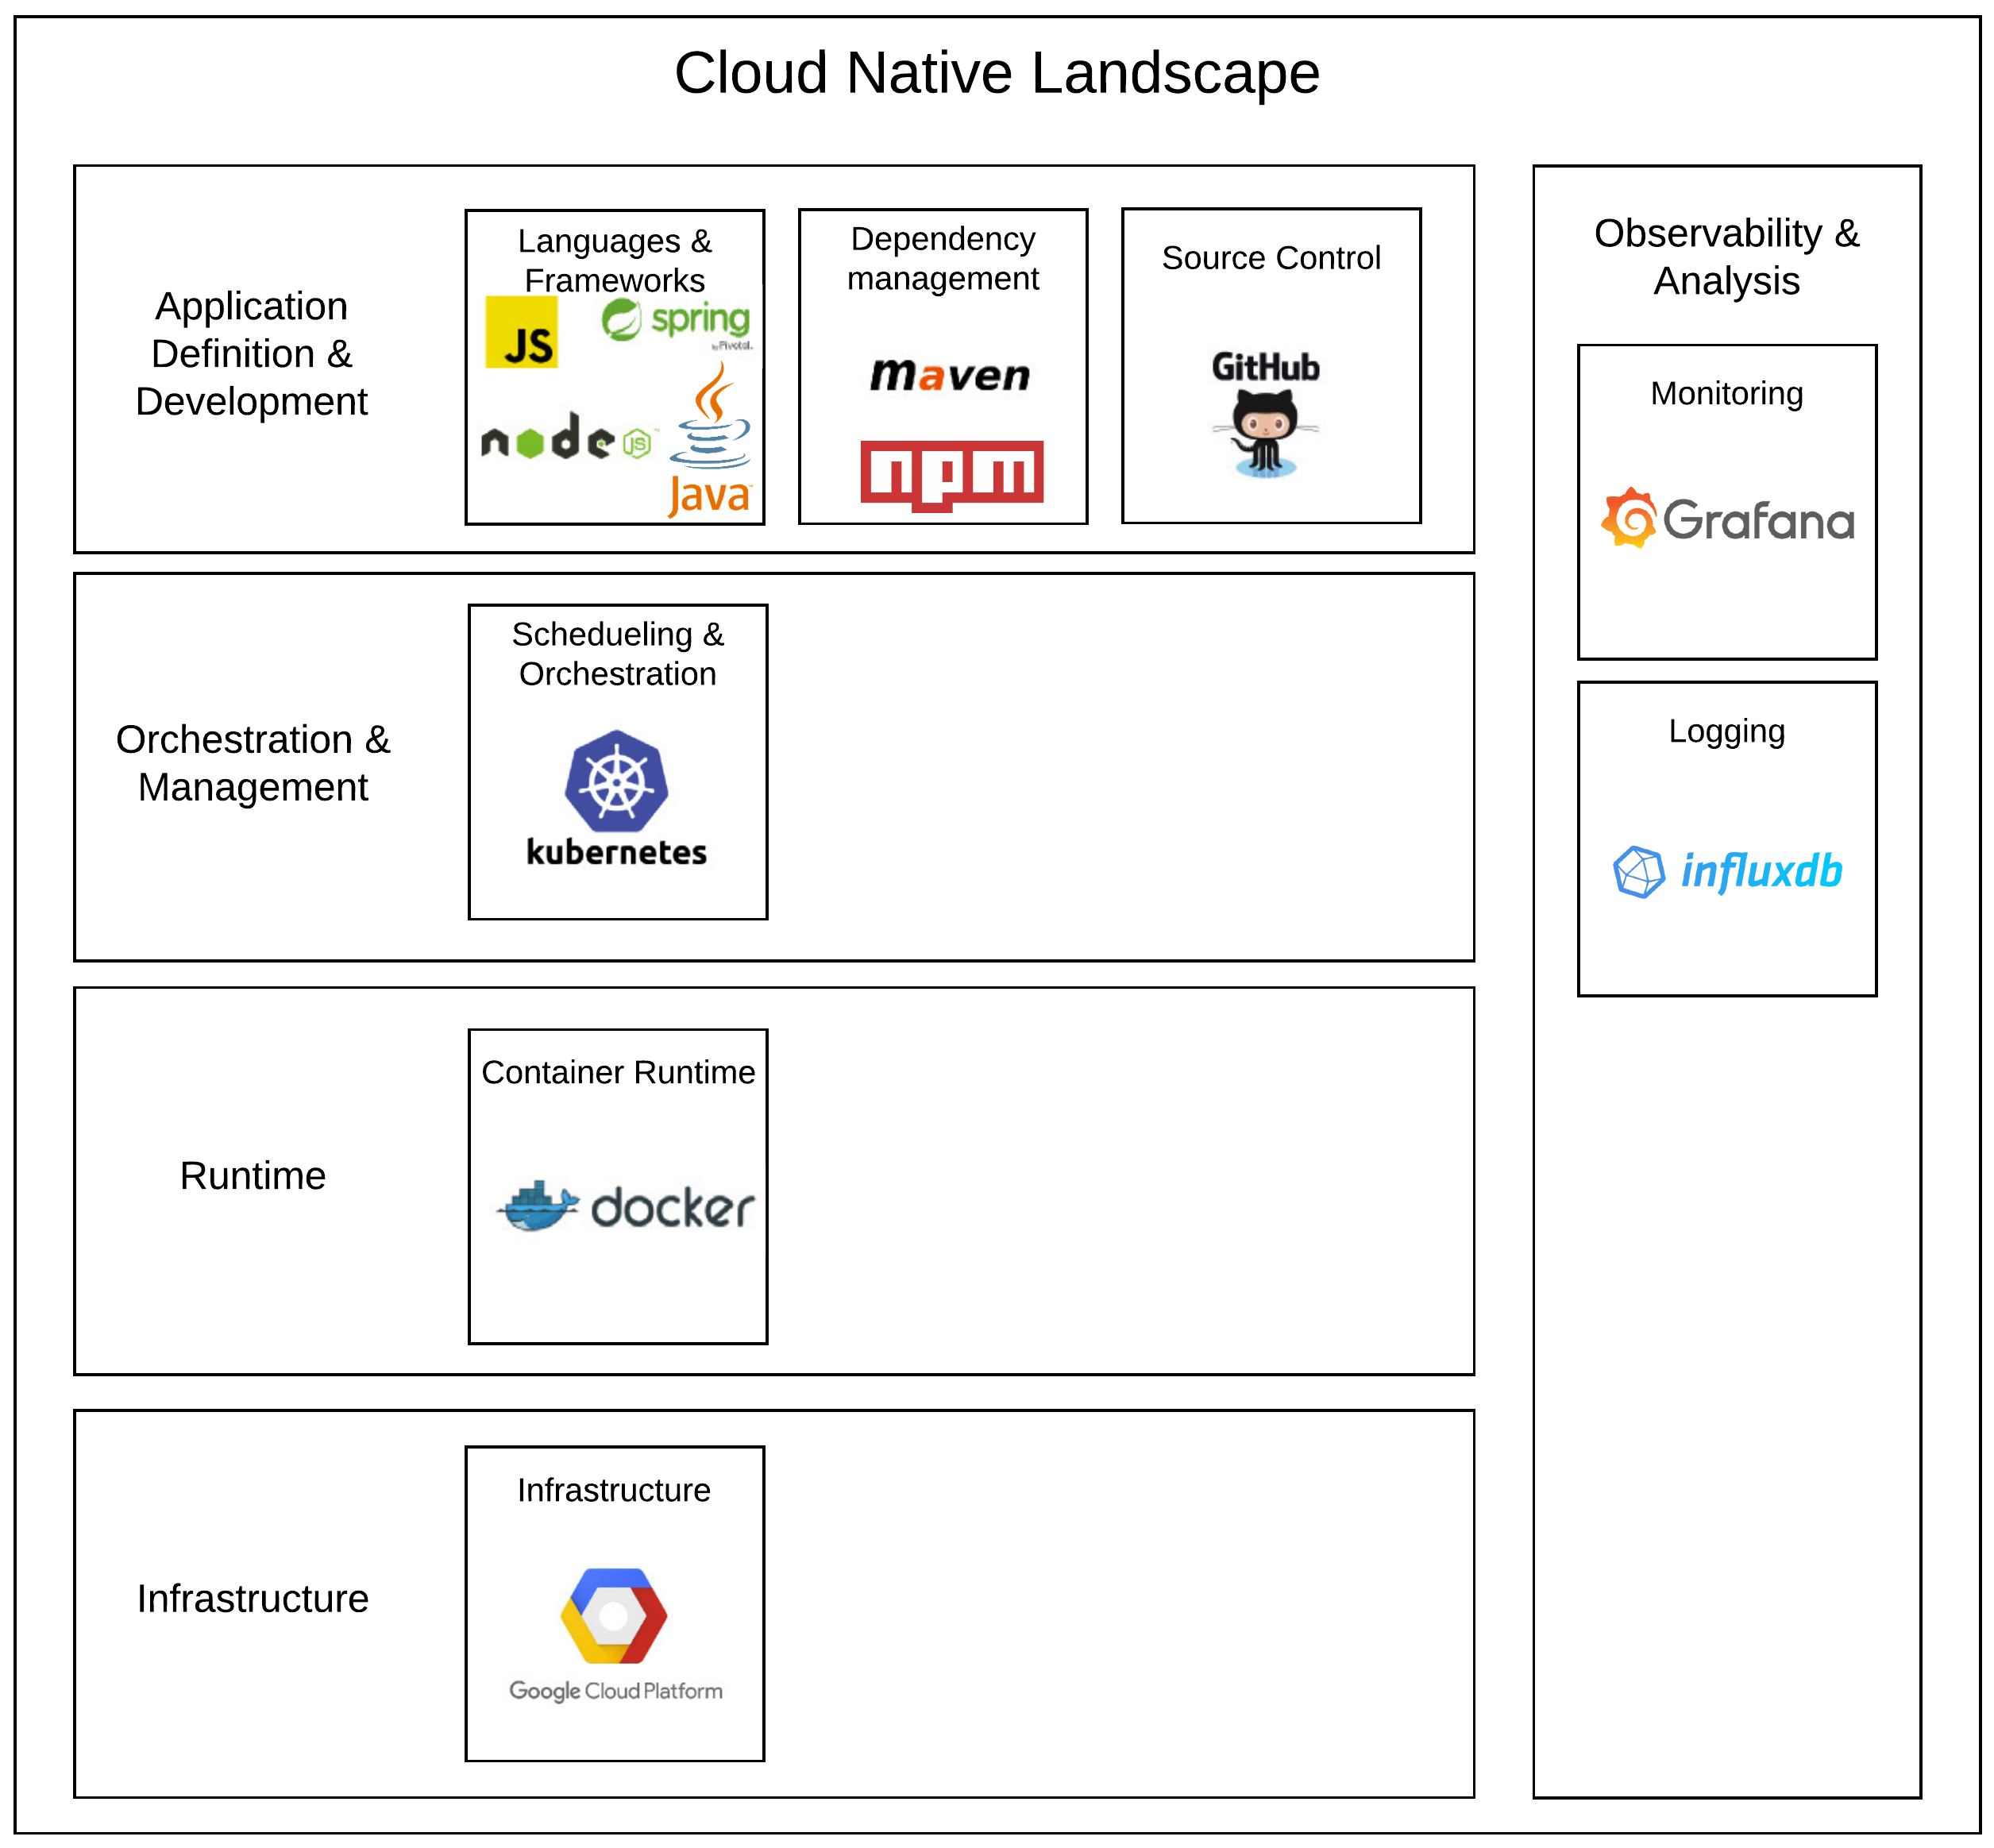
\includegraphics[scale=0.15]{cloud_computing_cloud_native_landscape}  
  \caption{The utilized technology stack, the entire Cloud Native Landscape can be found on: \url{https://github.com/cncf/landscape}}
  \label{fig:cloud_computing_cloud_native_landscape}
\end{center}
\end{figure}

\textbf{Infrastructure} \\
The provider, and the services they make available. The Google Cloud Platform infrastructure has been used extensively to host all experiments.

\textbf{Provisioning}\\ 
How the infrastructure is accessed and managed, and computing resources are reserved. No technologies have been utilized in this area, and it has therefore been omitted from the figure for the sake of simplicity.
 
\textbf{Runtime}\\
Runtime defines OS, storage, container runtime and networking. Docker has been used throughout all projects created and deployed during this thesis (see section \ref{sec:virtualization}).
 
\textbf{Orchestration \& Management}\\
Orchestration tools as well as services coordinating and management tools exist here. Kubernetes have been used for cluster creation and orchestration (see section \ref{sec:cluster}).
 
\textbf{Application Definition \& Development}\\
This level contains a lot of components. Here the application environment and its dependencies are listed including: databases, language and frameworks, source control management, dependency management, continuous integration (CI), continuous delivery (CD) among other aspects.

NodeJS is a JavaScript runtime webserver. NodeJS has been used to develop the test tool used in chapter \ref{ch:experiment}.

Spring Boot is a Java library that makes it possible to create Spring production-grade applications quickly. Spring Boot has been used to develop the test application load tested in chapter \ref{ch:experiment}.

\textbf{Observability \& Analysis}\\
This package contains tools that helps monitor and analyse system behaviour.

InfluxDB is the default time series database used in a Kubernetes cluster. InfluxDB is automatically set up to subscribe to event data from the cluster.

Grafana is the default time series analytics tool used in a Kubernetes cluster. Grafana visualizes data from the InfluxDB database in the cluster and provides a extensive user interface making it possible to monitor the cluster. Grafana has been utilized to gather data and monitor cluster configurations when conducting experiments.

\section{Virtualization, Hypervisors and Containers}
\label{sec:virtualization}
Resource pooling enables the remaining four essential characteristics of cloud computing: On-demand self-service, broad network access, rapid elasticity and measured service \cite{bittman2009server}. Resource pools are split  between consumers through a multitenancy layer that enables the cloud infrastructure to distribute one physical server between several consumers \cite{krebs2012architectural}. This multitenancy layer is created with hypervisor and container technologies that both provide virtualization, these technologies are fundamental for cloud computing. Virtualization makes it possible to create several emulations on one server that has the same attributes and characteristics as the physical system. This emulation has a memory address space, processor resources and device I/O, and is isolated from the rest of the system, utilizing its reserved amount of resources. This section will explain both technologies, their differences and why container technology has gained preference over VM's in the past few years.

\subsection{Hypervisors}
Hypervisors provide VM access to system resources. According to \cite[p.~100]{sosinsky2010cloud} two types of hypervisors exist, differentiated by whether the hypervisor is on top of a host OS or not.

\begin{itemize}
	\item \textbf{Type 1 Native:} The hypervisor has no host OS.
	\item \textbf{Type 2 Hosted:} The hypervisor is installed on top of a host OS (seen in Figure \ref{fig:cloud_computing_definition_virtualization}).
\end{itemize}

Type 1 VMs have no host operating system below them and are running directly on a bare system, completely simulating the hardware that it is running on. Type 1 virtualization is therefore called full virtualization. Type 2 VMs have an underlying host operating system, with a software interface mapping guest OSs system calls to the host OS. Hypervisor virtualization is machine-level virtualization, because it attempts to emulate a complete computing environment \cite{fink2014docker}. This makes this type of virtualization very resource intensive. A hypervisor approach is ideal when applications running on a single server require different OSs, and need access to a complete computing environment.

\begin{figure}[!htb]
	\centering 
		 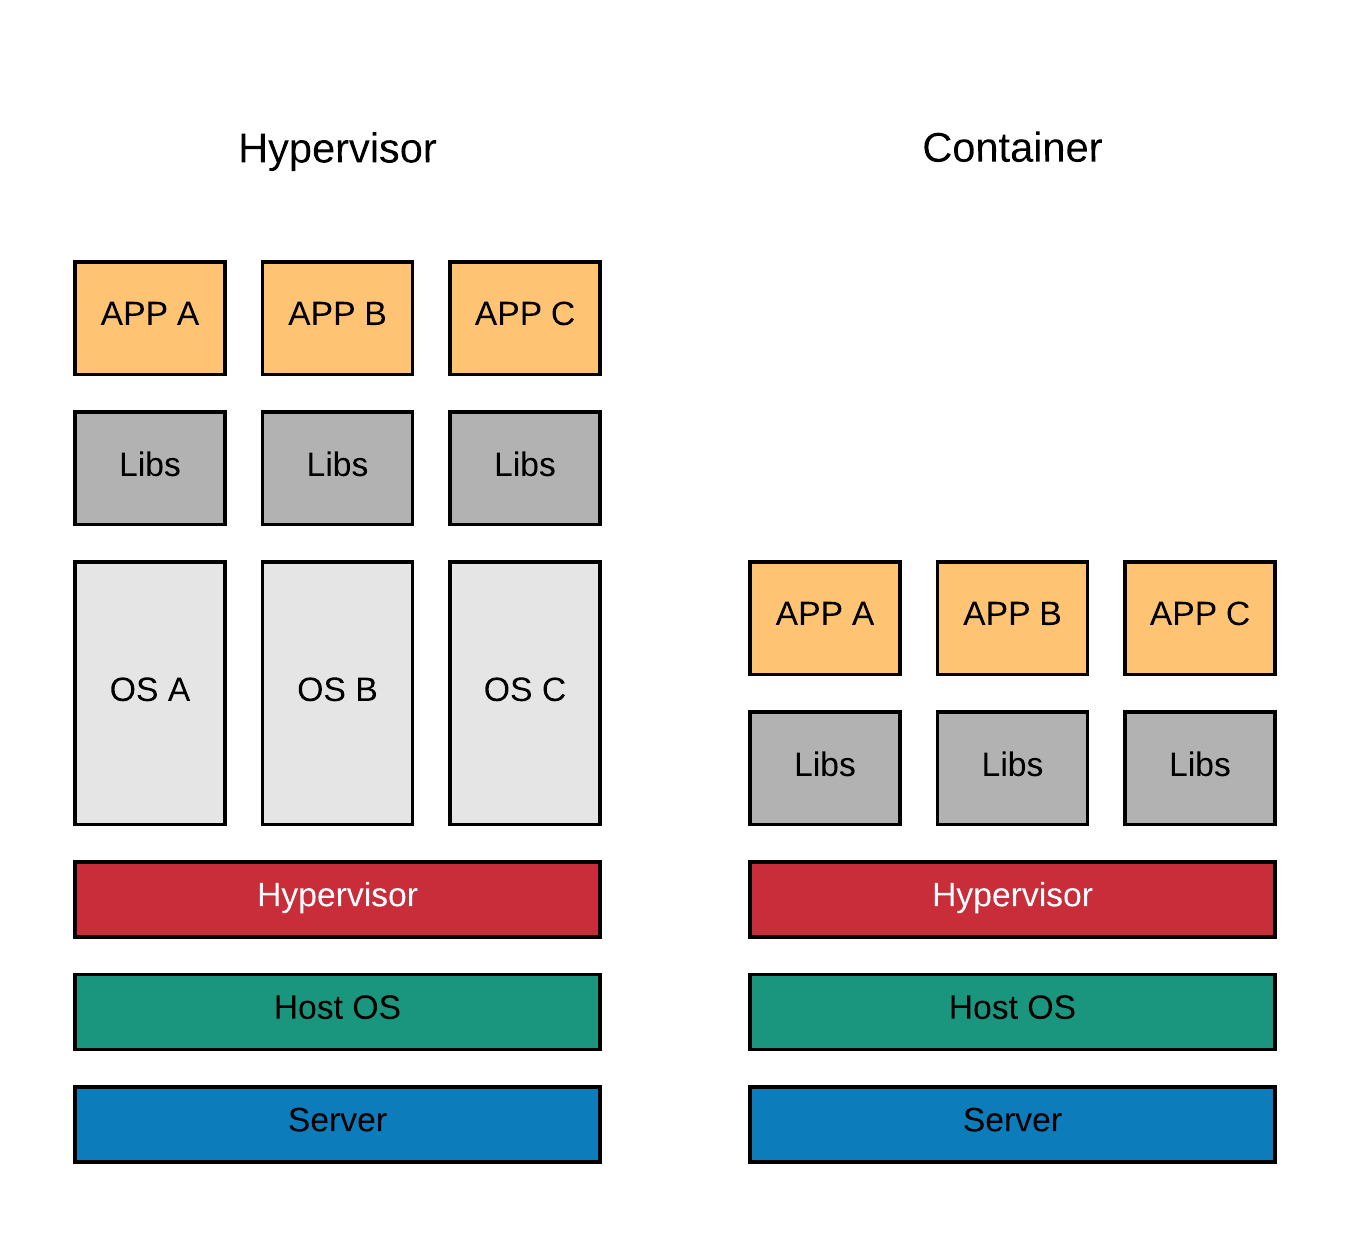
\includegraphics[scale=0.2]{cloud_computing_definition_virtualization}  
	  \caption{Hypervisor and container based deployment models \cite{bernstein2014containers}}
  \label{fig:cloud_computing_definition_virtualization}
\end{figure}

\subsection{Containers}
Containers always share OS with the host, container deployments are therefore very small, making it possible to have hundreds of containers running simultaneously on a single server. Containers try to share resources among running instances, by sharing RAM, disk space and kernel. Containers start up in seconds, while VMs take minutes to boot \cite{dockerFAQ}. Container virtualization is categorized as system-level virtualization, due to the containers operating at the process level. Container virtualization is known from the Linux kernel library Linux Container (LXC). LXC gives the possibility to create processes that are sand boxed from one another, controlling their available resources. Docker is the most popular container technology, utilizing LXC adding high-level tools on top. These tools further enhance container technology by improving usability and accessibility.

Due to containers natural small size, each service can be packed in its own container, providing excellent separation and isolation from other service executables, configurations, libraries and lifecycles. Each service can be packed separately, preventing services from affecting or conflicting with each other. Because each service doesn't need to be composed with the remaining services and is almost independent of the production environment (besides being the correct platform), immutable containers can be created \cite{kubernetes_what_is}. This gives a consistent environment from development into production, removing possible surprise challenges in the production environment.

\subsection{Comparison}
Figure \ref{fig:cloud_computing_definition_virtualization} compares a hypervisor and container approach. The hypervisor approach is ideal when different OS's or versions are needed, requiring a VM level abstraction\cite{bernstein2014containers}. Containers on the other hand reduce deployment size drastically, by utilizing a singular OS on each server. Even though the applications are limited to same platform as the server they are running on, containers have emerged as a very attractive virtualization method, due to very low overhead and ease of deployment \cite{fink2014docker}.

\note{
Resource pooling is in turn often enabled by the use of hypervisors or containers\cite{bernstein2014containers}. Common for both technologies is that they provide isolation and a multitenancy layer that enables the cloud infrastructure to serve different customers with one server instance\cite{krebs2012architectural}. By abstracting physical resources into virtual, management and automatic allocation of computing resource is made possible\cite{sosinsky2010cloud, armbrust2010view}, giving the possibility to subdivide physical resources, and present smaller and separate virtual resource partitions \cite{barham2003xen}. 

Supporting mordern development flow, where small pieces of code is written and tested in constant iteration \cite{fink2014docker}.

Modern applications often depend on many existing components, relying on other services and applications. These dependencies can easily conflict with other component dependencies\cite{merkel2014docker}. Using virtualization applications can be packaged along with dependencies and run in disparate environments, making distribution between development, test and production environments easy.
}

\subsection{Docker}
\label{sec:docker}
Docker is an open source project that provides developers with a high-level tool to manage container virtualization. Besides the earlier explained advantages with container virtualization itself, docker provides several benefits, making container virtualization even more usable. Docker introduces many indispensable features for big-scale application projects \cite{dockerFAQ}. The core features of docker are explained below:

\textbf{Portable Deployment across Machines}\\
By bundling the application with all its dependencies, and creating a machine-specific abstraction, docker makes it easy to run the exact same container on different machines with different configurations.

\textbf{Application-centric}\\
Docker centralizes the application in the deployment phase. Reducing friction when deploying the application. According to Burns et al. \cite{burns2016borg} this has several benefits, improving application deployment and introspection.

\textbf{Automatic Build}\\
Docker provides the dockerfile abstraction, making it possible to automatically assemble containers. A key feature for enabling many of the cloud infrastructure advantages. The dockerfile is a simple file that contains instructions about which libraries and deployment specific actions that are needed for successfully starting the containerized application.

\textbf{Versioning}\\
By introducing versioning of containers, docker makes it possible to track changes, introducing the many advantages known from git. Being able to see changes done to the container, control push of changes, introducing traceability all the way from development to production servers.

\textbf{Component Re-use}\\
The docker images support component re-use, a dockerfile can be used as base image in other dockerfiles, providing a base for more specialized components.

\textbf{Sharing}\\
Docker images are accessible on the Docker Hub, making it possible to share useful images, and take advantage of images shared. The docker hub also makes it possible to store images privately, still gaining the accessibility (eg. internally in an organisation) hindering outsiders from utilizing the image.

\textbf{Tool Ecosystem}\\
Docker makes it possible to automate and customize the creation and deployment of containers through a simple API.

\section{Cluster Management}
\label{sec:cluster}
Kubernetes is a container-management tool that watches for changes in the cluster, keeping it in a steady state \cite{burns2016borg}. Kubernetes is open source but has mainly been developed by Google that has extensive experience with running their infrastructure based on containers. Kubernetes has been developed with outset in two predecessor container-management tools developed internally by Google. Kubernetes main design goal is to ease deployment and management of complex distributed systems \cite{kubernetes_frontpage}. Kubernetes key features are described below:

\textbf{Automatic Binpacking}\\
Kubernetes places containers on servers according to the amount of resources needed by the container, maximizing utilization of server resources, with focus on availability.

\textbf{Self-Healing}\\
Containers are checked with user-defined health checks, making sure they are operating correctly. If not containers are killed and restarted, newly started containers are only advertised to users when ready to serve.

\textbf{Horizontal Scale}\\
Kubernets can scale service horizontally automatically and manually.

\textbf{Service Discovery and Load Balancing}\\
Containers are given a unique up address and a single DNS name, making them discoverable across the network.

\textbf{Automated Rollouts and Backups}\\
Rollouts of new configurations are done progressively while monitoring the application, making sure that there are some working instances at all times. Kubernetes can roll back configurations if working incorrectly.

\textbf{Storage Orchestration}\\
Kubernetes can automatically orchestrate storage, supporting local and remote storage options.


\section{Summary}
Many of cloud computings defining characteristics are tremendously important for microservices and therefore very interesting when looking at resilience in distributed applications. The container abstraction makes it possible to create truly separated environments, facilitating reproducibility and transparency. Cluster management gives us the ability to dynamically orchestrate containers adding more capacity and ensuring redundancy, improving the availability of a given system.